\phantomsection
\setcounter{secnumdepth}{3}

\setcounter{chapter}{1}
\chapter[{PHÂN TÍCH VÀ THIẾT KẾ HỆ THỐNG AGENT}]{Phân tích và Thiết kế Hệ thống Agent}

Chương này trình bày thiết kế hệ thống tác nhân cho bài toán điều khiển nhân vật trong môi trường game hành động Roguelike sinh bản đồ theo thủ tục. So với phiên bản thử nghiệm ban đầu chỉ điều khiển tác nhân cận chiến, hệ thống cuối cùng sử dụng CombatAgent: một tác nhân nhận quan sát dạng vector có cấu trúc, điều khiển di chuyển -- ngắm -- chiến đấu bằng không gian hành động rời rạc nhiều nhánh, và được huấn luyện trên nhiều mức độ khó thông qua học theo chương trình. Thiết kế này nhằm trả lời câu hỏi chính của khóa luận: làm thế nào để một chính sách PPO học được hành vi chiến đấu ổn định trong môi trường vừa có bản đồ thay đổi, vừa có tín hiệu thưởng thưa.

\section{Mô hình hóa bài toán dưới dạng MDP}

Theo mô hình học tăng cường đã trình bày ở Chương~1, bài toán được mô tả dưới dạng một Quy trình Quyết định Markov (Markov Decision Process -- MDP) với bộ thành phần $(S,A,P,R,\gamma)$ \cite{Schulman2017}. Tại mỗi bước quyết định, agent quan sát trạng thái hiện tại $s_t$, chọn hành động $a_t$, nhận phần thưởng $r_t$, sau đó môi trường Unity cập nhật sang trạng thái $s_{t+1}$ theo logic gameplay, vật lý 2D và cách sinh bản đồ.

Trong phạm vi khóa luận, $S$ là không gian quan sát vector của CombatAgent; $A$ là không gian hành động rời rạc nhiều nhánh gồm bốn nhánh; $R$ là hàm thưởng kết hợp giữa tín hiệu kết quả như tiêu diệt kẻ địch và tín hiệu định hình như tiếp cận mục tiêu; $\gamma=0.99$ là hệ số chiết khấu trong cấu hình PPO. Mục tiêu huấn luyện là tìm chính sách $\pi_{\theta}(a|s)$ tối đa hóa kỳ vọng tổng thưởng:

\begin{equation}
    J(\pi_\theta) = \mathbb{E}_{\tau \sim \pi_\theta}
    \left[\sum_{t=0}^{T}\gamma^t r_t\right].
\end{equation}

Điểm khó của bài toán nằm ở chỗ phân phối trạng thái thay đổi theo từng episode. Bản đồ được chọn từ nhiều text map khác nhau, vị trí spawn có thể cố định hoặc ngẫu nhiên theo lesson, kẻ địch và đạn di chuyển liên tục, còn phần thưởng hoàn thành phòng chỉ xuất hiện khi agent tiêu diệt đủ mục tiêu. Vì vậy, hệ thống cần một biểu diễn trạng thái đủ giàu để mô tả chiến đấu, nhưng vẫn đủ gọn để học hiệu quả bằng PPO.

\section{Không gian quan sát}

Hệ thống sử dụng quan sát dạng vector thay vì ảnh pixel. Lựa chọn này giúp giảm chi phí mẫu, tránh phải học lại các đặc trưng thị giác cơ bản, đồng thời phù hợp với mục tiêu nghiên cứu là đánh giá ảnh hưởng của học theo chương trình và các kỹ thuật khám phá trên một môi trường có cấu trúc. Trong Unity Inspector, kích thước quan sát vector của behavior CombatAgentConfig được cấu hình là 207 chiều.

\begin{table}[H]
    \centering
    \small
    \caption{Cấu trúc vector quan sát 207 chiều của CombatAgent}
    \label{tab:obs_207}
    \begin{tabular}{|p{4cm}|c|p{8cm}|}
        \hline
        \textbf{Nhóm quan sát} & \textbf{Số chiều} & \textbf{Nội dung chính} \\
        \hline
        Trạng thái người chơi & 13 & Máu, đạn, hồi chiêu, trạng thái sẵn sàng của vũ khí, tốc độ, sát thương gần đây, hướng vận tốc và padding để giữ kích thước cố định. \\
        \hline
        Thông tin toàn cục & 4 & Tỷ lệ kẻ địch nhìn thấy, tỷ lệ đạn nhìn thấy, thời gian episode đã chuẩn hóa và tín hiệu chết gần đây. \\
        \hline
        Kẻ địch gần nhất & 54 & 3 kẻ địch $\times$ 18 đặc trưng: vị trí tương đối, vận tốc tương đối, khoảng cách, máu, mức đe dọa, trạng thái tấn công, hồi chiêu và padding. \\
        \hline
        Đạn trong vùng nhìn & 120 & 10 viên đạn $\times$ 12 đặc trưng: vị trí tương đối, vận tốc, khoảng cách, thời gian ước lượng tới va chạm, loại chủ sở hữu và padding. \\
        \hline
        Tường/vật cản & 16 & 16 tia ray đều quanh agent, mỗi tia trả về khoảng cách chuẩn hóa tới tường gần nhất. \\
        \hline
        \textbf{Tổng} & \textbf{207} & $13 + 4 + 54 + 120 + 16 = 207$. \\
        \hline
    \end{tabular}
\end{table}

Thiết kế này cố ý tách rõ thông tin người chơi, kẻ địch, đạn và tường. Agent không cần suy luận vị trí đạn từ ảnh thô, nhưng vẫn phải học cách kết hợp nhiều nguồn nguy cơ: vừa tiếp cận kẻ địch để gây sát thương, vừa tránh đạn và không mắc vào tường. Vì số lượng kẻ địch và đạn trong scene có thể thay đổi, các block được giới hạn bởi MaxEnemies=3 và MaxBullets=10; nếu thiếu đối tượng thì hệ thống thêm giá trị 0 để vector luôn có kích thước cố định.

\section{Không gian hành động}

CombatAgent sử dụng không gian hành động rời rạc nhiều nhánh gồm bốn nhánh với kích thước $(3,3,3,9)$. Đây là điểm khác biệt quan trọng so với bản thử nghiệm cũ chỉ chọn một trạng thái FSM. Thay vì ra lệnh "đang di chuyển" hoặc "đang tấn công" ở mức thô, tác nhân trực tiếp chọn hướng di chuyển, ý định chiến đấu và hướng ngắm.

\begin{table}[H]
    \centering
    \small
    \caption{Không gian hành động rời rạc nhiều nhánh của CombatAgent}
    \label{tab:action_space}
    \begin{tabular}{|c|c|p{9cm}|}
        \hline
        \textbf{Branch} & \textbf{Kích thước} & \textbf{Ý nghĩa} \\
        \hline
        0 & 3 & moveX: không di chuyển theo trục X, sang trái, sang phải. \\
        \hline
        1 & 3 & moveY: không di chuyển theo trục Y, đi xuống, đi lên. \\
        \hline
        2 & 3 & combat: không hành động, tấn công, dash. Các lựa chọn tấn công hoặc dash có thể bị action mask khi vũ khí/kỹ năng chưa sẵn sàng. \\
        \hline
        3 & 9 & aim: giữ hướng cũ hoặc ngắm theo 8 hướng rời rạc. \\
        \hline
    \end{tabular}
\end{table}

Tổ hợp hai nhánh moveX và moveY tạo ra 9 hướng di chuyển (bao gồm đứng yên), trong khi nhánh aim điều khiển hướng tấn công. Entropy cực đại lý thuyết của không gian hành động, nếu mọi lựa chọn đều hợp lệ và phân phối đều, là:

\begin{equation}
    H_{\max} = \ln(3) + \ln(3) + \ln(3) + \ln(9) \approx 5.49 \text{ nat}.
    \label{eq:max_entropy}
\end{equation}

Giá trị này được dùng lại trong Chương~4 khi phân tích hiện tượng entropy plateau. Cần lưu ý rằng action mask có thể làm entropy cực đại thực tế thấp hơn tại một số trạng thái, vì các hành động như tấn công hoặc dash không phải lúc nào cũng hợp lệ.

\section{Thiết kế hàm phần thưởng}

Hàm thưởng được thiết kế theo hướng kết hợp sparse outcome reward và dense shaping reward \cite{Ibrahim2024}. Nhóm sparse reward phản ánh mục tiêu thật của phòng chơi, còn shaping reward cung cấp gradient trung gian để PPO không bị kẹt trong giai đoạn chưa từng hoàn thành phòng.

\begin{table}[H]
    \centering
    \small
    \caption{Các thành phần thưởng chính trong hai cấu hình reward}
    \label{tab:reward_components}
    \begin{tabular}{|p{4.4cm}|c|c|p{5.2cm}|}
        \hline
        \textbf{Sự kiện} & \textbf{v1} & \textbf{v2} & \textbf{Vai trò} \\
        \hline
        Gây sát thương & $+1.0$ & $+1.5$ & Khuyến khích tạo damage thay vì chỉ né tránh. \\
        \hline
        Hạ một kẻ địch & $+3.0$ & $+5.0$ & Tín hiệu kết quả thưa nhưng có ý nghĩa chiến thuật cao. \\
        \hline
        Dọn sạch toàn bộ phòng & $+5.0$ & $+10.0$ & Mục tiêu cuối của episode; reward v2 tăng mạnh tín hiệu hoàn thành. \\
        \hline
        Tiếp cận mục tiêu & $+0.008 \times \Delta d$ & $+0.003 \times \Delta d$ & Shaping khoảng cách, giảm ở v2 để tránh agent chỉ tối ưu tiếp cận. \\
        \hline
        Tấn công đúng hướng & $+0.05$ & $+0.15$ & Tăng reward cho ý định tấn công có căn chỉnh tốt. \\
        \hline
        Đứng gần địch không hành động & $-0.0005$ & $-0.002$ & Phạt hành vi chần chừ trong vùng nguy hiểm. \\
        \hline
        Agent chết & $-2.0$ & $-2.0$ & Tín hiệu terminal âm. \\
        \hline
    \end{tabular}
\end{table}

Bảng~\ref{tab:reward_components} chỉ liệt kê các thành phần chính. Trong hiện thực, code còn có các tín hiệu nhỏ hơn như time penalty, phạt nhận sát thương, thưởng dash hữu ích, phạt tấn công không hợp lệ và reward căn chỉnh hướng ngắm. Cấu hình v1 được dùng cho các run chính từ run34 đến run54. Cấu hình v2 được dùng trong run55 như một thí nghiệm thay đổi thang reward, vì vậy các giá trị mean reward của run55 không được so trực tiếp với các run v1.

\section{Sinh bản đồ bằng PCGNN và TilemapGenerator}

Môi trường huấn luyện dùng pipeline hai tầng. Tầng thứ nhất là PCGNN chạy offline ở phía Python để sinh nhiều bản đồ ứng viên từ một genome đã huấn luyện. Tầng thứ hai là TilemapGenerator trong Unity, có nhiệm vụ đọc các bản đồ văn bản đã được tuyển chọn, chuyển thành tilemap, chọn vị trí sinh và đưa phòng vào episode huấn luyện. Thiết kế này giữ được tính đa dạng của PCGNN nhưng tránh việc gọi Python trực tiếp trong mỗi episode Unity, nhờ đó giảm rủi ro latency và lỗi tích hợp trong quá trình train.

Mỗi bản đồ sau khi sinh được chuẩn hóa về định dạng văn bản của trò chơi: ký tự \texttt{\#} biểu diễn tường, \texttt{.} biểu diễn sàn, \texttt{P} là vị trí sinh người chơi và \texttt{E} là vị trí sinh kẻ địch. Vì output gốc của PCGNN chủ yếu là ma trận tile, đề tài bổ sung một adapter để đặt \texttt{P}/\texttt{E} trên cùng một thành phần liên thông của vùng sàn. Sau đó hệ thống chạy BFS để kiểm tra người chơi có thể đi tới kẻ địch hay không trước khi bản đồ được đưa vào tập huấn luyện.

\begin{figure}[H]
    \centering
    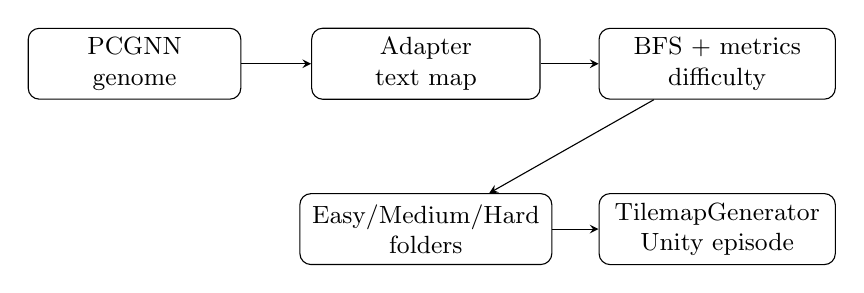
\begin{tikzpicture}[node distance=1.7cm, >=stealth, every node/.style={font=\small}]
        \node[draw, rounded corners, align=center, minimum width=2.7cm, minimum height=0.9cm] (pcgnn) {PCGNN\\genome};
        \node[draw, rounded corners, align=center, right of=pcgnn, xshift=2.0cm, minimum width=2.9cm, minimum height=0.9cm] (adapter) {Adapter\\text map};
        \node[draw, rounded corners, align=center, right of=adapter, xshift=2.0cm, minimum width=3.0cm, minimum height=0.9cm] (metric) {BFS + metrics\\difficulty};
        \node[draw, rounded corners, align=center, below of=adapter, yshift=-0.4cm, minimum width=3.2cm, minimum height=0.9cm] (tiers) {Easy/Medium/Hard\\folders};
        \node[draw, rounded corners, align=center, right of=tiers, xshift=2.0cm, minimum width=3.0cm, minimum height=0.9cm] (unity) {TilemapGenerator\\Unity episode};
        \draw[->] (pcgnn) -- (adapter);
        \draw[->] (adapter) -- (metric);
        \draw[->] (metric) -- (tiers);
        \draw[->] (tiers) -- (unity);
    \end{tikzpicture}
    \caption{Luồng sinh và tuyển chọn bản đồ bằng PCGNN trước khi đưa vào Unity}
    \label{fig:map_generation_workflow}
\end{figure}

Độ khó bản đồ được đánh giá bằng các chỉ số hình học gồm tỷ lệ tường, độ dài đường đi ngắn nhất giữa \texttt{P} và \texttt{E}, tỷ lệ ngõ cụt, tỷ lệ vùng có thể đi tới và độ khó A*. Thay vì đặt ngưỡng tuyệt đối cứng cho mọi generator, hệ thống có thể chia bản đồ theo thứ hạng tương đối: 5\% dễ nhất được đưa vào Easy, 5\% tiếp theo vào Medium và phần còn lại vào Hard. Cách chia này phù hợp với giai đoạn tuyển chọn thủ công vì người thiết kế vẫn có thể xem lại từng folder và chọn những bản đồ tốt nhất trước khi đưa sang Unity.

Trong Unity, TilemapGenerator không cần biết bản đồ được vẽ tay hay sinh bằng PCGNN. Thành phần này chỉ đọc text asset theo tier hiện tại, dựng tilemap và kiểm tra lại vùng có thể đi tới. Với các lesson dùng fixed spawn, TilemapGenerator ưu tiên ô sàn có độ phủ BFS tốt để tránh trường hợp player hoặc enemy bị cô lập. Với lesson dùng random spawn, player và enemy được chọn từ các ô sàn hợp lệ nhằm tăng phương sai môi trường.

\section{Khung curriculum learning}

Học theo chương trình được dùng để giảm độ khó khám phá ban đầu \cite{Bengio2009}. Thay vì đưa tác nhân ngay vào toàn bộ phân phối Hard, hệ thống bắt đầu từ bản đồ dễ hơn, chuyển sang Medium khi phần thưởng làm mượt vượt ngưỡng, rồi mới mở Hard. Tham số bài học được truyền qua Academy.Instance.EnvironmentParameters với tên difficulty.

\begin{figure}[H]
    \centering
    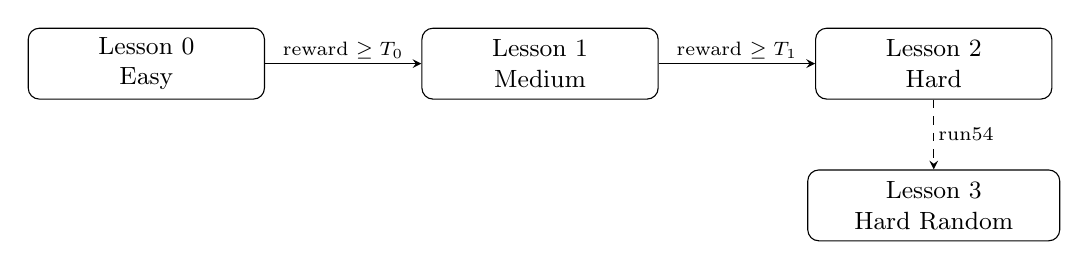
\begin{tikzpicture}[>=stealth,
        lesson/.style={draw, rounded corners, align=center, minimum width=3.0cm, minimum height=0.9cm, font=\small},
        transition/.style={font=\scriptsize, fill=white, inner sep=1.5pt}]
        \node[lesson] (easy) at (0,0) {Lesson 0\\Easy};
        \node[lesson] (medium) at (5.0,0) {Lesson 1\\Medium};
        \node[lesson] (hard) at (10.0,0) {Lesson 2\\Hard};
        \node[lesson, minimum width=3.2cm] (random) at (10.0,-1.8) {Lesson 3\\Hard Random};
        \draw[->] (easy.east) -- node[transition, above]{reward $\geq T_0$} (medium.west);
        \draw[->] (medium.east) -- node[transition, above]{reward $\geq T_1$} (hard.west);
        \draw[->, dashed] (hard.south) -- node[transition, right]{run54} (random.north);
    \end{tikzpicture}
    \caption{Cấu trúc curriculum 3-tier và biến thể 4-tier fixed-to-random}
    \label{fig:curriculum_structure}
\end{figure}

Trong run46, curriculum gồm 3 lesson: Easy, Medium và Hard. Trong run54, curriculum được mở rộng thành 4 lesson: Easy Fixed, Medium Fixed, Hard Fixed và Hard Random. Biến thể 4-tier kiểm tra giả thuyết rằng việc giảm phương sai spawn ở giai đoạn đầu có thể giúp PPO ổn định hơn trước khi chuyển sang phân phối khó hơn.

\section{Kiến trúc mạng nơ-ron}

Chính sách được huấn luyện bằng PPO trong Unity ML-Agents \cite{Juliani2018}. Cấu hình baseline dùng mạng MLP actor-critic với hidden\_units=256, num\_layers=2, normalize=true. Actor head sinh phân phối xác suất cho bốn branch hành động, còn critic head ước lượng $V(s)$ để tính advantage theo GAE.

\begin{figure}[H]
    \centering
    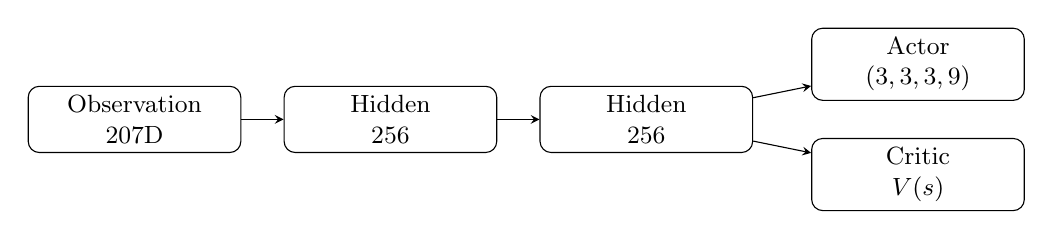
\begin{tikzpicture}[node distance=1.45cm, >=stealth, every node/.style={font=\small}]
        \node[draw, rounded corners, align=center, minimum width=2.7cm] (obs) {Observation\\207D};
        \node[draw, rounded corners, align=center, right of=obs, xshift=1.8cm, minimum width=2.7cm] (h1) {Hidden\\256};
        \node[draw, rounded corners, align=center, right of=h1, xshift=1.8cm, minimum width=2.7cm] (h2) {Hidden\\256};
        \node[draw, rounded corners, align=center, right of=h2, xshift=2.0cm, yshift=0.7cm, minimum width=2.7cm] (actor) {Actor\\$(3,3,3,9)$};
        \node[draw, rounded corners, align=center, right of=h2, xshift=2.0cm, yshift=-0.7cm, minimum width=2.7cm] (critic) {Critic\\$V(s)$};
        \draw[->] (obs) -- (h1);
        \draw[->] (h1) -- (h2);
        \draw[->] (h2) -- (actor);
        \draw[->] (h2) -- (critic);
    \end{tikzpicture}
    \caption{Kiến trúc actor-critic dùng cho CombatAgentConfig}
    \label{fig:actor_critic_architecture}
\end{figure}

Một số run ablation bổ sung bộ nhớ LSTM với memory\_size=256 và sequence\_length=64 để kiểm tra giả thuyết rằng thông tin lịch sử có thể giúp agent xử lý đạn, hồi chiêu và tình huống khuất tầm nhìn. Kết quả định lượng của các lựa chọn kiến trúc này được trình bày ở Chương~4.
